\chapter{Wybrane technologie}

W tym rozdziale opisane zostaną technologie użyte do rozwiązania zadanego problemu.
System został podzielony na różne komunikujące się ze sobą aplikacje i każda z nich
wymaga różnego podejścia do ich wytworzenia. Z tego powodu ten rozdział został podzielony
na podrozdziały, każdy z nich opisujący dany program i technologie użyte do ich
utworzenia.

\section{Aplikacja kliencka}
Aplikacja kliencka została wykonana w formie strony internetowej.

\subsection*{WebAssembly}
WebAssembly\cite{webassembly} to technologia opisująca standardowy kod binarny oraz jego reprezentację tekstową,
niezależne od platformy jego wykonania \cite{mdn:wasm, wasm:standard}. Umożliwia to
tworzenie przenośnego oprogramowania, które może zostać wykorzystane w wielu różnych systemach.
Głównymi celem WebAssembly jest umożliwienie tworzenia szybkiego oraz bezpiecznego pod względem
obsługi pamięci oprogramowania, które może być stworzone w dowolnym języku programowania, 
niezależnie od platformy oraz sprzętu, na którym ma być wykonywane \cite{wasm:standard}.

\subsection*{Rust}
Rust\cite{rust} to wielo-paradygmatowy kompilowany język programowania. Oznacza to, że łączy ze sobą cechy różnych
konwencje wielu sposobów tworzenia oprogramowanie m.in. programowanie obiektowe, funkcjonalne
czy strukturalne i umożliwia osobie je tworzącej na korzystanie z dowolnych zasobów oraz
schematów danego paradygmatu. 

Celem tego języka jest umożliwienie tworzenia wydajnego oprogramowania jednocześnie
dbając o bezpieczeństwo pamięci oraz konkurencji \cite{infoworld:what_is_rust}. 
Uzyskane jest to poprzez wykorzystanie mechanizmu sprawdzania zapożyczeń (ang. \textit{borrow checker}).
Mechanizm ten sprawdza czas życia danego obiektu podczas kompilacji co sprawia, że nie wymagane
jest to podczas działania oprogramowania w przeciwieństwie do systemów z klasycznym zliczaniem referencji.
Dzięki temu nie jest wymagane użycie algorytmów odśmiecania pamięci
(ang. \textit{garbage collection}) lub zliczania referencji (ang. \textit{reference counting}), 
które dodają dodatkowe koszty wykonywania obliczeń.

Środowisko programistyczne Rust zapewnia również wiele przydatnych narzędzi
ułatwiających tworzenie oprogramowania \cite{klabnik:rust}.
Jednym z nich jest serwer języka rust-analyzer, który może zostać zintegrowany
z wieloma popularnymi środowiskami deweloperskimi oraz edytorami tekstu,
w celu zapewnienia dodatkowych funkcjonalności takie jak
autouzupełnianie czy wyświetlanie błędów kompilacji podczas edycji kodu.
Kolejnym z nich jest oprogramowanie Cargo spełniające dwie główne funkcje - 
jest systemem budującym projekt oraz umożliwia na zarządzanie zależnościami.
Pozwala to na łatwe umieszczanie kodu innych publicznie dostępnych projektów
w oprogramowaniu docelowym oraz wykorzystywanie jego funkcjonalności.

Cechy te sprawiają, że ten język programowania regularnie cieszy się z
wysokiego zadowolenia użytkowników w rankingach StackOverflow.
W roku 2022 9,32\% respondentów używało języka Rust i aż 86,73\% z nich
uznało, że kocha z nim pracować \cite{stackoverflow:popularity}.
Jest to najwyższy wynik z jakiejkolwiek technologii w tej ankiecie,
drugie miejsce zajmuje język Elixir z wynikiem 75,46\%. 
Dane te przedstawiono na Rys. \ref{stack:loved}.
Dzięki tak dużej popularności powstało wiele otwarto-źródłowych bibliotek,
które mogą pomóc w rozwiązaniu zadanego problemu.
\begin{figure}[!htb]
  \centering
  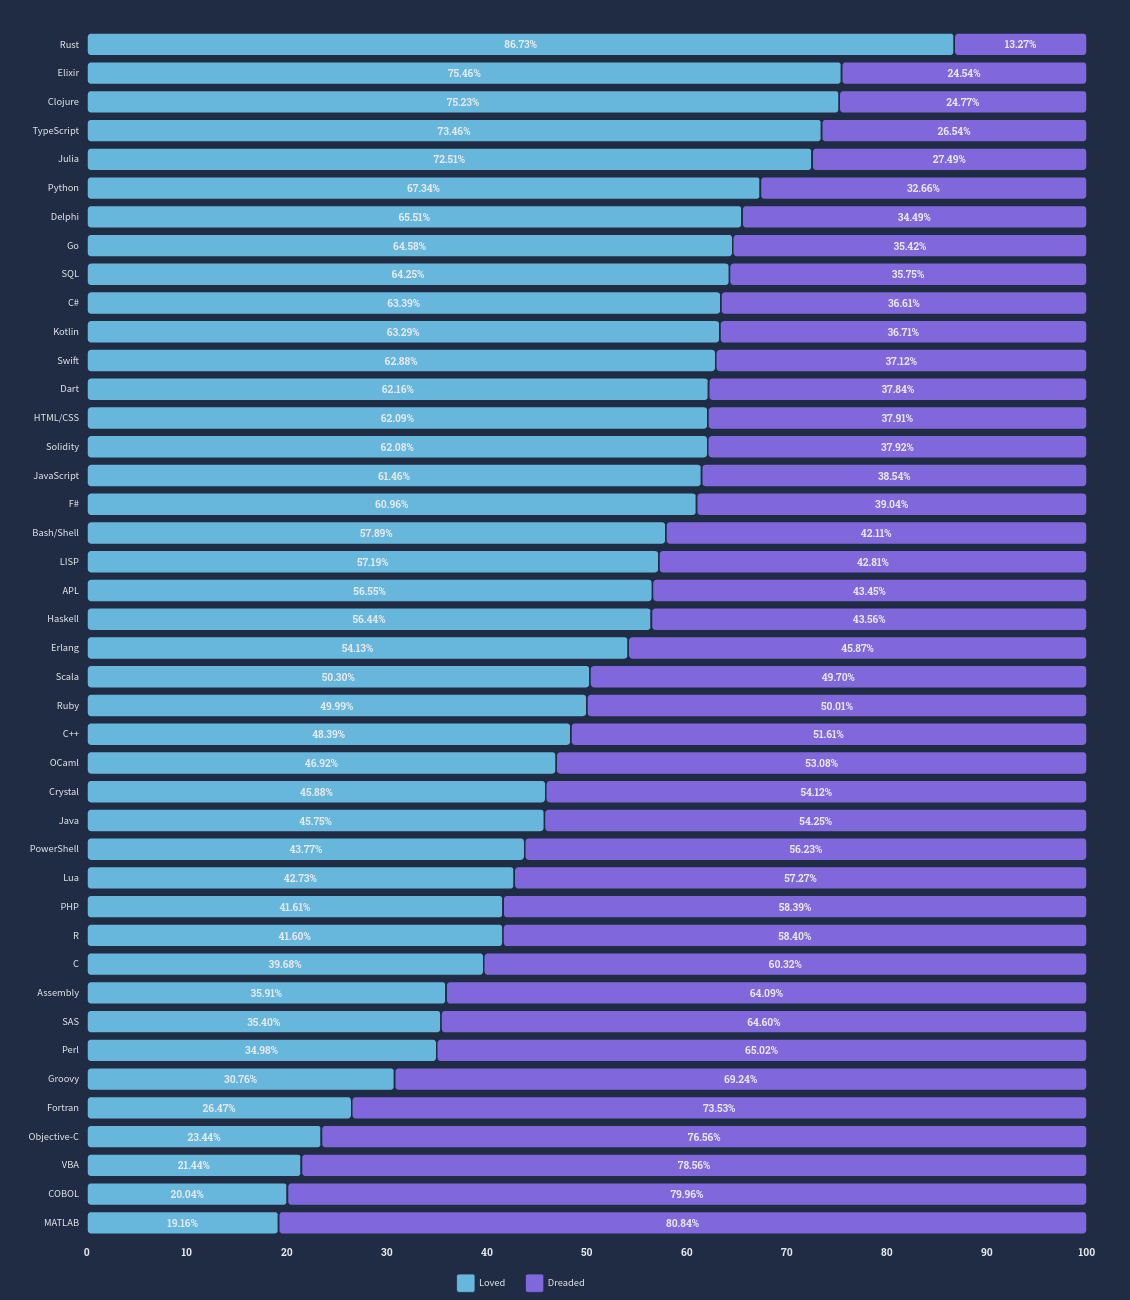
\includegraphics[width=\textwidth]{stack_loved}
  \caption{Wykres przedstawiający współczynnik uwielbiania/nienawiści danej technologii}
  \label{stack:loved}
  \caption*{Źródło: \url{https://survey.stackoverflow.co/2022}}
\end{figure}
\FloatBarrier

\subsection*{Yew}
Yew\cite{yew} to framework umożliwiający tworzenie witryn WWW w języku Rust.
Z użyciem tej biblioteki możliwe jest konstruowanie niezawodnych
oraz wydajnych stron internetowych. Yew wykorzystuje WebAssembly wraz
z renderowaniem po stronie serwera, aby znacznie przyśpieszyć działanie
aplikacji na docelowej platformie. Umożliwia również na wykorzystanie 
funkcjonalności innych popularnych języków wykorzystywanych do tworzenia
aplikacji webowych takich jak JavaScript poprzez wykorzystanie biblioteki
wasm-bindgen udostępniającej standardową funkcjonalność tego języka oraz
pozwalającą na połączenie ze skryptami stworzonymi w tym języku.

Do tworzenia stron Yew wykorzystuje język podobny do HTML i JSX dzięki
czemu jest przystępny dla programistów mających wcześniejsze doświadczenie
z tymi technologiami. Podobnie jak inne środowiska takie jak React czy Angular
tworzone są komponenty, które mogą być wielokrotnie używane w różnych komponentach
oraz podstronach co sprawia, że kod jest czytelniejszy, zmniejszona jest jego złożoność
oraz możliwe jest wyeliminowanie niepotrzebnych powtórzeń.

Platforma umożliwia na wykorzystanie wielu jej rozszerzeń. Jedną z nich jest biblioteka
yew-hooks pozwalająca na wykorzystanie tzw. haczyków umożliwiających na 
funkcjonalność taką jak dynamiczne odświeżanie danych, wykonywanie operacji
asynchronicznych czy obserwowanie zmian zmiennych i reagowanie na nie.
Kolejną jest wasm-bindgen pozwalająca na generowanie połączeń z szeroko stosowanym
w tworzeniu aplikacji webowych językiem JavaScript. Umożliwia na stosowanie
funkcjonalności tego języka jak również generowaniu dwustronnych połączeń między
środowiskami - w skryptach JavaScript możliwe jest wywoływanie kodu napisanego
w języku Rust i na odwrót.

\subsection*{Bootstrap}
Bootstrap\cite{bootstrap} to darmowe i otwarto-źródłowe środowisko programistyczne składające się
ze zbioru szablonów stworzonych w językach HTML, CSS i JavaScript, które mogą
być dowolnie wykorzystane z kompatybilnymi technologiami.
Ten framework zawiera podstawowe style potrzebne, aby stworzyć responsywną 
aplikacje webowe na wielu urządzeniach z różnymi rozmiarami ekranów oraz rozdzielczością. 
Dzięki zastosowaniu systemu flex bardzo usprawnia rozmieszczanie elementów na stronie
oraz dostosowanie ich rozmiaru czy zachowania.

\subsection*{TypeScript}
TypeScript\cite{typescript} to darmowy, otwarto źródłowy stworzony oraz utrzymywane przez przedsiębiorstow Microsoft.
Jest rozszerzeniem popularnego języka JavaScript dodającym szeroko zastosowane funkcjonalności
w innych statycznie typowanych językach, tj. adnotacje typów oraz ich sprawdzanie
podczas kompilacji, interfejsy, typy wyliczeniowe czy uogólnienia.
Dodatkowo rozszerza język o słowa kluczowe async/await ułatwiające pracę
z asynchronicznymi funkcjami. Język TypeScript jest całkowicie kompatybilny ze 
środowiskami wspierającymi JavaScript - jest to język kompilowany do języka JavaScript, a
dodatkowe funkcjonalności dostępne są jedynie podczas tworzenia oprogramowania.

Jego wykorzystanie w aplikacji zostało ograniczone jedynie do wykonania funkcjonalności,
których implementacja w pozostałych technologiach była niemożliwa lub znacznie 
utrudniona. Są to głównie funkcje pomocnicze wywoływane w odpowiednich komponentach
stworzonych w technologii Yew.

\section{Aplikacja serwerowa}

\subsection*{.NET Core}
.NET Core\cite{netcore} to następca popularnej platformy programistycznej .NET Framework stworzonej przez
firmę Microsoft. W przeciwieństwie do poprzednika, którego oficjalne wsparcie ograniczone było
do systemu Windows, a same oprogramowanie było własnościowe, jest to technologia otwarto-źródłowa
wspierająca wiele systemów operacyjnych \cite{price2021c}. Możliwe jest to poprzez zastosowanie
języka pośredniego niezależnego od systemu lub sprzętu. Instrukcje te tłumaczone są w 
wirtualnej maszynie CLR (ang. \textit{Common Language Runtime}) na język maszynowy, a
następnie wykonywane jak standardowy natywny kod \cite{msdn:clr}. Dzięki takiemu podjeściu
możliwe jest wytworzenie przenośnego oprogramowania, które może być wykorzystane na wielu
systemach.

\subsection*{C\#}
C\#\cite{csharp} to silnie typowany język obiektowy wysokiego poziomu stworzony przez firmę Microsoft.
Do kompilacji wykorzystywane jest środowisko .NET, dzięki czemu zachowane są
jego cechy takie jak przenośność oprogramowania oraz możliwość wykorzystania
innych języków programowania bazujących na tej technologii.

Dzięki automatycznemu zarządzaniu pamięcią ułatwia znacznie tworzenie
oprogramowania, gdyż w bezpiecznym kontekście nie pozwala na 
błędne jej wykorzystanie. Wykonywane jest to poprzez zastosowanie
mechanizmu odśmiecania pamięci (ang. \textit{garbage collection}).

C\# zawiera również rozszerzenia kolekcji LINQ (ang. \textit{Language Integrated Query})
pozwalające na wykonywanie na nich dodatkowych operacji, tj. grupowanie, sortowanie czy wyszukiwanie.
Te dodatkowe metody mogą być wykorzystane do działań na róznych źródłach danych takich jak dokumenty XML
czy też bazy danych SQL \cite{zhang2014}. Ich wysokopoziomowy kod jest przenośny i może być
wykorzystywany w takiej samej formie przy różnych źródłach danych.

Kolejną zaletą tej technologii jest możliwość wykorzystania meta-programowania. 
Jest to technika umożliwiająca modyfikację kodu podczas jego kompilacji lub wykonywania. 
Dzięki niej podczas wykonywania programu, poprzez refleksję, możliwe jest rozpoznanie
typu obiektu oraz jego modyfikacja. Pozwala również na tworzenie drzew wyrażeń, które
mogą zostać dynamicznie skompilowane w celu, np. wykorzystania zaawansowanej logiki
biznesowej, która może być zmienna.

\subsection*{ASP.NET}
ASP.NET\cite{aspnet} to modularna platforma programistyczna oparta na technologii .NET. 
Jej bogata funkcjonalność pozwala na tworzenie stron internetowych, API HTTP oraz 
wiele innych aplikacji webowych poprzez zastosowanie wielu z jej rozszerzeń.
Jednym z nich jest wstrzykiwanie zależności (ang. \textit{dependency injection})
pozwalające na uzyskanie rozwiązania podobnego do wzorca architektury inwersji
kontroli (ang. \textit{Inversion of Control}). W takiej architekturze, zamiast
polegać na szczegółowej implementacji danej funkcjonalności czy serwisu,
użytkownik otrzymuje interfejs mówiący jedynie o tym do czego jest on przeznaczony.
Dzięki temu uzyskany kod jest całkowicie oddzielny od implementacji i pozwala
na znaczne ograniczenie efektów ubocznych przy działaniach takich jak refaktoryzacja,
restrukturyzacja czy przenoszenie implementacji, aby ta korzystały z innej biblioteki, np.
przy zmianie systemu bazodanowego.

Poprzez zastosowanie tak zwanych pośredników (ang. \textit{Middleware}) ASP.NET udostępnia
bardzo modularną oraz modyfikowalną strukturę przetwarzania zapytań HTTP.
Są to proste kroki, w których wykonywana jest logika związana z zapytaniem lub odpowiedzią
wysyłaną przez serwer. Podczas ich wykonania możliwy jest dostęp do danych zawartych
w zapytania oraz następnie jego modyfikacja, jak również decyzja o tym czy powinno
być ono propagowane do dalszych warstw. Przydatne to jest w przypadku, np. autoryzacji
gdzie w module sprawdzającym tożsamość użytkownika możliwe jest modyfikacja oraz zwrócenie
odpowiedzi o nieautoryzowanym dostępie i nie przekazywanie zapytania dalej do warstw, które zajmują
się dostępem do danych. Możliwe jest również zastosowanie innych pośredników takich
jak przechowywanie zapytań oraz odpowiedzi na nie w pamięci podręcznej, co znacznie
zwiększa wydajność systemu przy wielu takich samych zapytaniach. Poza wieloma wbudowanymi
pośrednikami programista sam może definiować swoją własną logikę oraz umieszczać
ją w odpowiednim momencie łańcucha wykonania.

\subsection*{MongoDB}
MongoDB\cite{MongoDB} to wieloplatformowy system bazodanowy. Dane przechowywane są w postaci dokumentów,
w formacie podobnym do JSON (ang. \textit{JavaScript Object Notation}), określaną nazwą
BSON (ang. \textit{Binary JSON}). Główną różnicą między tymi formatami jest sposób kodowania
danych - w przypadku formatu JSON jest to postać znaków UTF-8, a BSON jest to zapis binarny.
Pozwala to na łatwą konwersję między tymi typami, czyli co za tym idzie również uzyskiwanie
czytelnych dla człowieka danych, tym samym oszczędzając miejsce potrzebne do przechowywania
informacji jak również przyśpieszenie niektórych operacji jak indeksowanie.

W porównaniu do klasycznych baz danych SQL, MongoDB pozwala na większą elastyczność dzięki braku
konieczności określania schematu tabel. Wszystkie schematy są dynamiczne i mogą w dowolnym momencie 
zostać zmienione w celu dodania dodatkowych informacji jednocześnie nie zmieniając pozostałych
danych zapisanych w danej kolekcji. Jednocześnie ten system pozwala na tworzenie 
walidatorów kolekcji, co przydaje się w momentach kiedy chcemy uzyskać większą kontrolę
nad strukturą danych.

\subsection*{Docker}
Docker\cite{docker} to zbiór oprogramowania umożliwiający dystrybucję oprogramowania jako tzw. kontener.
Są to wyspecjalizowane maszyny wirtualne, zawierające jedynie oprogramowanie potrzebne
do uruchomienia danego rozwiązania. Podobnie jak zwykłe rozwiązania wirtualizacyjne
są one od siebie odizolowane, ale w przeciwieństwie do innych, klasycznych rozwiązań
działają one na tym samym jądrze systemu operacyjnego dzięki czemu zużywają znacznie
mniej zasobów\cite{docker:what_is_container}. Odpowiednio skonfigurowane połączenia
między maszynami umożliwiają komunikację, np. poprzez protokół TCP. 
Po odpowiednim spakowaniu obrazu ta technologia umożliwia wykorzystanie identycznego
oprogramowania w różnych środowiskach niezależnie od systemu operacyjnego hosta.

Oprogramowaniem, które wchodzi w skład tego kompleksu i zostało ekstensywnie wykorzystane 
w realizacji projektu jest docker-compose. Te narzędzie wykorzystuje pliki konfiguracyjne
w formacie YAML, aby ułatwić pracę w środowiskach wymagających użycia kliku kontenerów, np.
w przypadku aplikacji serwerowej, która ma komunikować się z bazą danych. Przy użyciu
jednej komendy możliwe jest zbudowanie oraz wdrożenie całej infrastruktury systemu.
Możliwe jest również aktualizowanie pojedynczych aplikacji wchodzących w jego skład 
bez stopowania reszty systemu.

\section{Urządzenie pomiarowe}
Urządzenie pomiarowe wykonane zostało na płytce Raspberry Pi Pico W, do którego z wykorzystaniem
portów ogólnego przeznaczenia GPIO podłączono sensory badające parametry środowiska, 
które następnie są przetwarzane oraz przesyłane na serwer.

\subsection*{Raspberry Pi Pico W}
Raspberry Pi Pico W\cite{picow} to komputer jedno-płytkowy zbudowany na podstawie mikrokontrolera RP2040. 
Do głównych jego cech, które zostały wykorzystane do stworzenia systemu należą \cite{rp2040:datasheet}:
\begin{itemize}
  \item procesor dwurdzeniowy ARM Cortex-M0+,
  \item 264kB pamięci SRAM,
  \item 2MB pamięci flash,
  \item kontroller DMA (ang. \textit{Direct memory access}),
  \item 30 pinów GPIO (ang. \textit{General-purpose input/output}),
  \item 2 kontrollery SPI (ang. \textit{Direct memory access}),
  \item 2 kontrollery I2C (ang. \textit{Serial Peripheral Interface}),
  \item 16 kanałów PWM (ang. \textit{Pulse-width modulation}).
\end{itemize}
Płytka umożliwia łączność z siecią Wi-Fi przy użyciu wbudowanego chipu CYW43439
obsługujący standard 802.11n, który w odpowiednich warunkach pozwala na łączność
z prędkością do 600Mb/s. Wraz z nowszymi wersjami SDK umożliwia również wykorzystanie
całego potencjału tego urządzenia i umożliwia na połączenia protokołem Bluetooth.
Dzięki zastosowanym komponentom to urządzenie jest zdolne do relatywnie szybkiego 
przetwarzania danych, przy niskim zużyciu energii. Dodatkowo wiele portów I/O umożliwia
na podłączenie wielu różnych sensorów, jednak w wypadku wykorzystania wielu z nich
należy zwracać uwagę na szybkość wykonywania operacji, gdyż przy większej ilości akcji
system może je przetwarzać w czasie większym niż spodziewany. Jednak atrakcyjna cena urządzenia,
ustanowiona przez producenta jako 4 USD umożliwia na wykorzystanie kilku z nich w jednej instalacji
bez większych kosztów.

Aktualnie dostępne oprogramowanie pozwala tworzyć systemy w językach programowania takich jak
Assembly, C, C++, Python oraz Rust. Istnieje również nieoficjalne wsparcie dla środowiska
Arduino oraz możliwość wykorzystania istniejących na tą platformę bibliotek.
Ze względu na język, w którym utworzono SDK (ang. \textit{Software Development Kit}) dla
tej platformy (język programowania C), najczęściej wykorzystywane są języki C oraz C++
ze względu na wysoki stopień kompatybilności.

\subsection*{C++}
C++\cite{isocpp} to obiektowy język programowania wysokiego poziomu, będący często określany jako
rozszerzenie języka C często używanego do tworzenia oprogramowania na systemy wbudowane.
Obsługuje on wysokopoziomowe abstrakcje takie jak obiekty, programowanie generyczne czy
abstrakcje pozwalając w tym samym czasie na używanie niskopoziomowej funkcjonalności 
takiej jak zarządzenie pamięcią czy dostęp do rejestrów procesora oraz używanie języka asembler.
Przez te cechy używany jest tam, gdzie potrzebna jest wysoka wydajność lub zasoby komputerowe
są znacznie ograniczone, np. serwery WWW, gry komputerowe czy systemy wbudowane.

W porównaniu do C zawiera również rozbudowaną standardową bibliotekę klas i funkcji.
Dodaje ona dodatkową funkcjonalność taką jak zaawansowane typy pozwalające na
przechowywanie zmiennej liczby danych, algorytmy takie jak sortowanie czy 
generowanie liczb losowych, obsługa plików, czasu oraz wielowątkowości.
Inną dużą zaletą tego języka jest możliwość wykorzystania wszystkich bibliotek napisanych
w języku C co nie koniecznie musi być prawdziwe w drugą stronę - programista musi
udostępnić specjalny interfejs, aby wykorzystać kod stworzony w języku C++
w programach stworzonych w C.
